%% -*- TeX-engine: xetex; TeX-master: "draft.tex"; ispell-dictionary: "russian" -*-

\section{Количественная оценка модели}

\subsection{Сравнение с существующими моделями}
\label{sub:comparison}

В качестве метода для сравнения мы выбрали  MSC (см.~\ref{subsub:msc}), так как
он ближе всего к предлагаемой модели. Алгоритм MSC использует два состояния, поэтому
мы уменьшили множество состояний переключающейся мультиномиальной СММ до двух, объединив
состояния \texttt{LOW} и \texttt{HIGH} в одно --- \texttt{METHYLATED}.

Результаты работы обоих методов сравнивались на данных бисульфитного секвенирования
стволовых клеток мыши. Допустимое количество ошибок для состояния $\texttt{METHYLATED}$
было ограничено 1\%. Результаты сравнения для трёх первых хромосом генома мыши приведены в
таблице~\ref{table:comparison}. В последней колонке таблицы указано количество метилированных
цитозинов, которые были найдены обеими моделями.
\begin{table}[htbp!]
  \centering
  \begin{tabular}{lrrrr}
    \textbf{Хромосома} & \textbf{MSC} & \textbf{MSHMM} & \textbf{Пересечение} \\
    \noalign{\nobreak\smallskip}
    chr1 & 1136756 & 1291624 & 1136756 \\
    chr2 & 1114488 & 1316179 & 1114488 \\
    chr3 & 896377  & 1040715 & 896377
  \end{tabular}
  \caption{Количество метилированных цитозинов по мнению алгоритма MSC и
    переключающейся мультиномиальной СММ (MSHMM).}
  \label{table:comparison}
\end{table}

\vspace{-7pt}
Получается, что результаты переключающейся мультиномиальной СММ полностью
включают результаты алгоритма MSC, что не удивительно, так как предлагаемая модель
является строгим обобщением биномиальной смеси, используемой в алгоритме MSC.


\subsection{Анализ генов <<домашнего хозяйства>>}
\label{sub:housekeeping}

Гены <<домашнего хозяйства>> (housekeeping genes) --- это гены, необходимые для
поддержания жизнедеятельности клетки в организме. Они активны на всех стадиях
жизненного цикла организма. Одним из необходимых условий активности гена является
отсутствие метилирования в начале гена и в участке до его начала \cite{Jones2012}.

С помощью переключающейся мультиномиальной СММ был проведён анализ метилирования генов
<<домашнего хозяйства>> в мыши (табл.~\ref{tab:housekeeping}). Ожидалось, что у всех
десяти рассматриваемых генов не будет обнаружено метилирование.

\begin{table}[htbp!]
  \centering
  \begin{tabular}{cc}
    \textbf{Идентификатор RefSeq} & \textbf{Символ гена} \\
    \noalign{\nobreak\smallskip}
    NM\_007393 & ACTB \\
    NM\_008951 & PSMD4 \\
    NM\_023372 & RPL38 \\
    NM\_025344 & EIF3F \\
    NM\_026069 & RPL37 \\
    NM\_026885 & CHMP2A \\
    NM\_133691 & PUF60 \\
    NM\_172736 & LENG8 \\
    NM\_172757 & HEATR8 \\
    NM\_198033 & SETX
  \end{tabular}
  \caption{Список генов <<домашнего хозяйства>> в мыши \cite{Kouadjo2007}. Для каждого
    гена приведён соответствующий символ (gene symbol) и идентификатор в базе данных NCBI
    RefSeq.}
  \label{tab:housekeeping}
\end{table}

В результате из десяти генов, у восьми не было отмечено наличие метилирования в начале гена
(рис.~\ref{fig:heatr3}), а два гена начинались с гипометилированного участка (рис.~\ref{fig:setx}).

\begin{figure}[htbp!]
  \centering
  \begin{subfigure}{\textwidth}
    \centering
    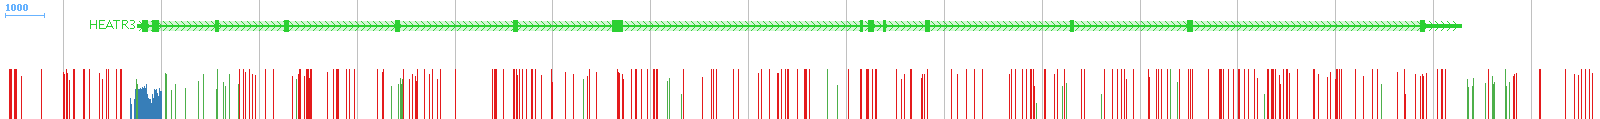
\includegraphics[width=\textwidth]{images/HEATR3}
    \caption{HEATR3}
    \label{fig:heatr3}
  \end{subfigure}
  \par\bigskip
  \begin{subfigure}{\textwidth}
    \centering
    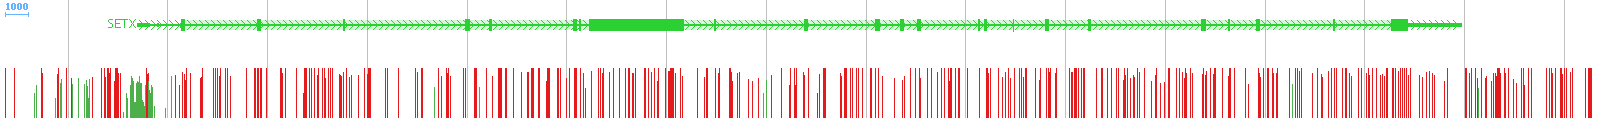
\includegraphics[width=\textwidth]{images/SETX}
    \caption{SETX}
    \label{fig:setx}
  \end{subfigure}
  \caption{Результаты работы переключающейся мультиномиальной СММ на генах <<домашнего хозяйства>> мыши.}
\end{figure}

На основании проведённых экспериментов можно предполагать, что полученная модель биологически
интерпретируема: на восьми из десяти рассмотренных генов <<домашнего хозяйства>> мыши модель
показала результаты, которые соответствуют описанным ожиданиям.
